% =====================================================================
% Brown bag seminar — story arc version
% Story: canonical global games -> why LLMs -> LLMs play canonical game
%        -> communication raises participation -> surveillance lowers action
%        -> beliefs don't move.
% Compile from slides/: pdflatex brown_bag.tex
% =====================================================================
\documentclass[aspectratio=169,12pt]{beamer}

\usetheme{default}
\setbeamertemplate{navigation symbols}{}
\setbeamertemplate{footline}{%
  \hfill\usebeamercolor[fg]{page number in head/foot}\insertframenumber/\inserttotalframenumber\hspace{0.4cm}\vspace{0.2cm}}

\usepackage{amsmath, amssymb}
\usepackage{graphicx}
\usepackage{booktabs}
\usepackage{array}
\usepackage{tikz}
\usetikzlibrary{arrows.meta, positioning, shapes.geometric, calc}
\usepackage{xcolor}

% Graduate Center / CUNY-inspired palette
% Primary GC/CUNY blue from gc.cuny.edu theme CSS: #005DAB
\definecolor{paper}{HTML}{FFFFFF}
\definecolor{purple}{HTML}{005DAB}   % primary GC/CUNY blue; keep command name for existing markup
\definecolor{accent}{HTML}{FE5000}   % GC orange accent
\definecolor{teal}{HTML}{1AB0DC}     % GC cyan accent
\definecolor{warn}{HTML}{D13176}     % GC magenta/pink accent for surveillance/warnings
\definecolor{good}{HTML}{237457}     % GC green accent
\definecolor{muted}{HTML}{586F82}    % GC slate
\definecolor{dark}{HTML}{2E312F}     % GC near-black body text
\definecolor{soft}{HTML}{E7F1F4}     % pale GC blue background

\setbeamercolor{background canvas}{bg=paper}
\setbeamercolor{normal text}{fg=dark,bg=paper}
\setbeamercolor{frametitle}{fg=paper,bg=purple}
\setbeamercolor{title}{fg=purple}
\setbeamercolor{subtitle}{fg=muted}
\setbeamercolor{author}{fg=purple}
\setbeamercolor{institute}{fg=muted}
\setbeamercolor{date}{fg=muted}
\setbeamercolor{alerted text}{fg=warn}
\setbeamercolor{block title}{fg=paper,bg=purple}
\setbeamercolor{block body}{fg=dark,bg=soft}
\setbeamercolor{alertblock title}{fg=paper,bg=warn}
\setbeamercolor{alertblock body}{fg=dark,bg=soft}
\setbeamercolor{itemize item}{fg=accent}
\setbeamercolor{itemize subitem}{fg=teal}
\setbeamercolor{enumerate item}{fg=accent}
\setbeamerfont{frametitle}{size=\Large,series=\bfseries}
\setbeamerfont{title}{size=\LARGE,series=\bfseries}
\setbeamerfont{subtitle}{size=\large}

\newcommand{\hl}[1]{{\color{accent}\textbf{#1}}}
\newcommand{\bad}[1]{{\color{warn}\textbf{#1}}}
\newcommand{\ok}[1]{{\color{good}\textbf{#1}}}
\newcommand{\m}[1]{{\color{muted}#1}}
\newcommand{\takeaway}[1]{\begin{block}{Takeaway}\small\raggedright #1\end{block}}
\newcommand{\bigclaim}[2]{\begin{center}{\LARGE\color{#1}\textbf{#2}}\end{center}}

\title{LLMs Can Play (Global) Games}
\subtitle{Natural-language coordination, validation, and extensions}
\author{Khaled Eltokhy}
\institute{CUNY Graduate Center, Department of Economics}
\date{Brown bag seminar --- April 2026}

\begin{document}

% 1 -------------------------------------------------------------------
\begin{frame}[plain]
  \vspace{1.0cm}
  {\usebeamerfont{title}\color{purple}\inserttitle\par}
  \vspace{0.35cm}
  {\usebeamerfont{subtitle}\color{muted}\insertsubtitle\par}

  \vfill
  {\large\color{purple}\insertauthor}\par
  {\color{muted}\insertinstitute}\par
  {\color{muted}\insertdate}\par
\end{frame}

% 2 -------------------------------------------------------------------
\begin{frame}{The story in five steps}
  \large
  \begin{enumerate}\setlength\itemsep{0.45em}
    \item Start with a \hl{canonical global game}.
    \item Embed the private signal in \hl{natural language}.
    \item Show LLM actions reproduce the \hl{Morris--Shin threshold pattern}.
    \item Validate the signal channel: \hl{scramble collapses, flip reverses}.
    \item Then use the laboratory for extensions: communication and surveillance.
  \end{enumerate}
\end{frame}

% 3 -------------------------------------------------------------------
\begin{frame}{A coup game: coordination creates multiplicity}
  \normalsize
  Following the standard coup-game framing: citizens want to participate only if the uprising succeeds; success requires participation above a threshold.

  \medskip
  \centering
  \renewcommand{\arraystretch}{1.18}
  \begin{tabular}{c|cc}
    & \textbf{Uprising succeeds} & \textbf{Uprising fails} \\
    \hline
    \textbf{Join} & $B$ & $-C$ \\
    \textbf{Stay} & $0$ & $0$ \\
  \end{tabular}

  \medskip
  \begin{columns}[T]
    \begin{column}{0.48\textwidth}
      \begin{block}{Strategic complementarity}
        \small Joining is attractive when I expect many others to join.
      \end{block}
    \end{column}
    \begin{column}{0.48\textwidth}
      \begin{alertblock}{Selection problem}
        \small Because each person's best response depends on expected participation, both mass joining and mass abstention can be self-confirming.
      \end{alertblock}
    \end{column}
  \end{columns}
\end{frame}

% 4 -------------------------------------------------------------------
\begin{frame}{Enter global games}
  \normalsize
  Global games make the payoff-relevant fundamental uncertain and privately observed.

  \medskip
  \begin{itemize}\setlength\itemsep{0.35em}
    \item Nature draws \hl{$\theta$}, the regime's strength.
    \item Lower $\theta$: easier to topple. Higher $\theta$: harder to topple.
    \item Citizen $i$ sees a noisy private signal:
      \[
        x_i=\theta+\varepsilon_i,\qquad \varepsilon_i\sim\mathcal N(0,\sigma^2).
      \]
    \item Agents infer both the fundamental and what others are likely to have seen.
  \end{itemize}

  \smallskip
  {\small\color{muted}\textbf{Key move:} noisy private signals generate a unique cutoff equilibrium: join when the signal says the regime is weak enough.}
\end{frame}

% 5 -------------------------------------------------------------------
\begin{frame}{Canonical continuum version}
  \footnotesize
  Each citizen in a continuum chooses $a_i\in\{0,1\}$, where $a_i=1$ means JOIN; $\theta$ is the normalized participation threshold.

  \vspace{0.03cm}
  \begin{block}{Aggregate participation and success}
    \centering
    $A\equiv \int_0^1 a_i\,di$ \qquad and \qquad $\text{uprising succeeds} \iff A>\theta$.
  \end{block}

  \vspace{0.03cm}
  Morris--Shin's result is a unique monotone equilibrium:
  \begin{block}{Threshold rule}
    \centering\normalsize
    $\text{join} \iff x_i < x^*$
  \end{block}

  \vspace{0.03cm}
  \begin{itemize}\setlength\itemsep{0.08em}
    \item Lower signal $x_i$ means a weaker-looking regime.
    \item The cutoff $x^*$ is common in equilibrium and pinned down by marginal-agent indifference.
    \item Aggregate joining therefore falls as regime strength rises.
  \end{itemize}
\end{frame}

% 6 -------------------------------------------------------------------
\begin{frame}{Prediction for the LLM experiment}
  \small
  If citizens follow the cutoff rule, aggregate joining is pinned down by the distribution of private signals:
  \[
    A(\theta)=\Pr(x_i<x^*\mid \theta)=\Phi\left(\frac{x^* - \theta}{\sigma}\right).
  \]

  \vspace{-0.1cm}
  \centering
  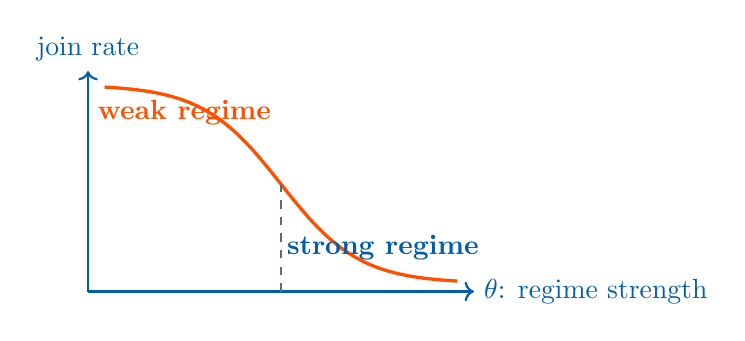
\begin{tikzpicture}[scale=0.70]
    \draw[->, thick, color=purple] (0,0) -- (7,0) node[right] {$\theta$: regime strength};
    \draw[->, thick, color=purple] (0,0) -- (0,4) node[above] {join rate};
    \draw[very thick, color=accent, domain=0.3:6.7, samples=100] plot (\x,{3.6/(1+exp(1.4*(\x-3.5)))+0.15});
    \draw[dashed, thick, color=muted] (3.5,0) -- (3.5,2.0);
    \node[color=accent, font=\bfseries] at (1.75,3.25) {weak regime};
    \node[color=purple, font=\bfseries] at (5.35,0.8) {strong regime};
  \end{tikzpicture}

  \vspace{-0.05cm}
  {\small\color{muted}\textbf{Empirical test:} as $\theta$ rises, fewer signals fall below $x^*$, so JOIN rates should decline like $\Phi((x^*-\theta)/\sigma)$.}
\end{frame}

% 7 -------------------------------------------------------------------
\begin{frame}{Why LLMs make this a clean laboratory}
  \begin{columns}[T]
    \begin{column}{0.48\textwidth}
      \textbf{Human subjects}
      \begin{itemize}\setlength\itemsep{0.25em}
        \item costly at scale
        \item have memory across rounds
        \item hard to rewrite information environment cleanly
        \item difficult to expose to many counterfactual regimes
      \end{itemize}
    \end{column}
    \begin{column}{0.48\textwidth}
      \textbf{LLM calls}
      \begin{itemize}\setlength\itemsep{0.25em}
        \item stateless calls: no memory unless we give it
        \item natural language information, not just numbers
        \item exogenous prompt manipulation
        \item identical game under censorship/surveillance/placebo variants
      \end{itemize}
    \end{column}
  \end{columns}

  \medskip
  \begin{alertblock}{Interpretation}
    \small
    The claim is not that LLMs are citizens; it is that they let us test controlled comparative statics in a rich language environment.
  \end{alertblock}

  \vspace{-0.15cm}
  {\tiny\color{muted}Related: Horton (2023), ``Large Language Models as Simulated Economic Agents,'' NBER WP 31122.}
\end{frame}

% 8 -------------------------------------------------------------------
\begin{frame}{The LLM experiment}
  \centering
  \resizebox{0.96\textwidth}{!}{%
  
\begin{tikzpicture}[node distance=0.65cm, every node/.style={font=\small}]
    \node[draw=purple, very thick, rounded corners, fill=soft, minimum width=2.5cm, minimum height=0.9cm] (theta) {$\theta$};
    \node[draw=purple, very thick, rounded corners, fill=soft, minimum width=2.5cm, minimum height=0.9cm, right=of theta] (signal) {$x_i=\theta+\varepsilon_i$};
    \node[draw=purple, very thick, rounded corners, fill=soft, minimum width=2.7cm, minimum height=0.9cm, right=of signal] (brief) {briefing};
    \node[draw=purple, very thick, rounded corners, fill=soft, minimum width=2.7cm, minimum height=0.9cm, right=of brief] (llm) {LLM call};
    \node[draw=accent, very thick, rounded corners, fill=soft, minimum width=2.7cm, minimum height=0.9cm, right=of llm] (decision) {JOIN/STAY};
    \draw[-{Latex[length=3mm]}, thick, color=purple] (theta) -- (signal);
    \draw[-{Latex[length=3mm]}, thick, color=purple] (signal) -- (brief);
    \draw[-{Latex[length=3mm]}, thick, color=purple] (brief) -- (llm);
    \draw[-{Latex[length=3mm]}, thick, color=purple] (llm) -- (decision);
  \end{tikzpicture}%
  }

  \medskip
  \normalsize
  The continuous signal becomes a private natural-language intelligence briefing.

\end{frame}

% 9 -------------------------------------------------------------------
\begin{frame}{Example: signal embedded in prose}
  \small
  \begin{quote}
  \textbf{PRIVATE BRIEFING}\par
  \textbf{BOTTOM LINE:} The regime's cohesion is visibly fraying.\par
  \textbf{ATMOSPHERE:} Street talk has shifted from complaint to anticipation.

  \medskip
  \textbf{EVIDENCE:}
  \begin{itemize}
    \item[--] Security forces show friction and delays.
    \item[--] Business families are moving capital with urgency.
    \item[--] Graffiti appeared overnight and has not been cleaned.
  \end{itemize}
  \end{quote}

  \bigskip
  \takeaway{No payoff numbers. No explicit $\theta$. The strategic signal is carried by language.}
\end{frame}

% 10 ------------------------------------------------------------------
\begin{frame}{Baseline result: LLMs play the canonical global game}
  \centering
  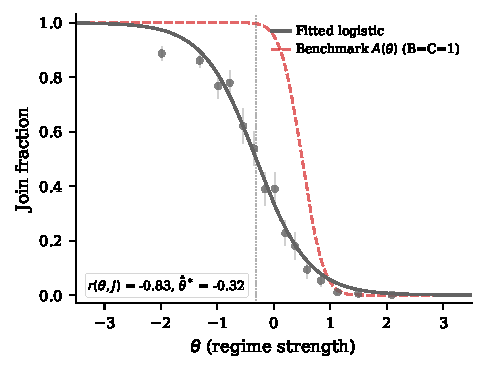
\includegraphics[height=0.64\textheight]{../paper/figures/fig01_sigmoid.pdf}

  \smallskip
  \normalsize
  Join rates move with the latent fundamental and follow the predicted decreasing sigmoid.
\end{frame}

% 11 ------------------------------------------------------------------
\begin{frame}{Validation: not just generic sentiment}
  \centering
  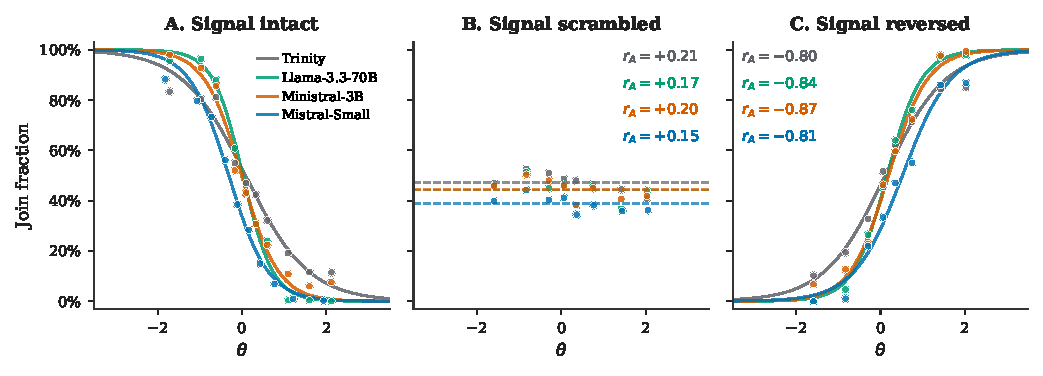
\includegraphics[width=0.94\textwidth]{../paper/figures/fig03_falsification.pdf}

  \medskip
  \begin{itemize}\setlength\itemsep{0.25em}
    \item \textbf{Pure}: threshold relationship appears.
    \item \textbf{Scramble}: destroy signal assignment, relationship collapses.
    \item \textbf{Flip}: reverse signal content, relationship flips.
  \end{itemize}
\end{frame}

% 12 ------------------------------------------------------------------
\begin{frame}{Extension 1: allow citizens to communicate}
  \large
  Canonical model: \hl{signals $\to$ actions}.\par
  \medskip
  Extension: \hl{signals $\to$ peer messages $\to$ actions}.\par

  \medskip
  \normalsize
  \begin{itemize}\setlength\itemsep{0.3em}
    \item Agents send short messages to neighbours before choosing JOIN/STAY.
    \item Decision-stage agent sees its own briefing plus neighbours' messages.
    \item The communication channel can reveal what others know.
  \end{itemize}
\end{frame}

% 13 ------------------------------------------------------------------
\begin{frame}{Extension 1 result: communication raises participation}
  \centering
  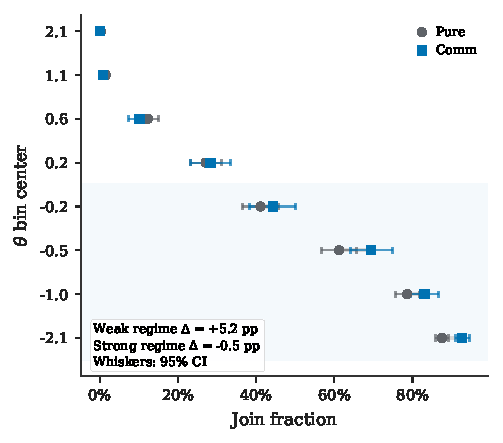
\includegraphics[height=0.60\textheight]{../paper/figures/fig05_communication.pdf}

  \smallskip
  \bigclaim{good}{Participation rises when agents can talk.}
\end{frame}

% 14 ------------------------------------------------------------------
\begin{frame}{Why communication should matter}
  \Large
  In a global game, my private signal is useful.\par
  \bigskip
  But your message helps me infer \hl{what others are likely seeing and doing}.\par

  \bigskip
  \begin{block}{Interpretation}
    Communication partly converts private information into shared information, making coordinated action easier.
  \end{block}
\end{frame}

% 15 ------------------------------------------------------------------
\begin{frame}{Extension 2: monitor the communication channel}
  \large
  Add one sentence to the \hl{messaging prompt}:

  \bigskip
  \begin{alertblock}{Surveillance warning}
  \small
  ``You have reason to believe that your communications are being monitored by regime security services, and messages deemed subversive could have serious consequences for you and your contacts.''
  \end{alertblock}

  \bigskip
  \textbf{The decision prompt is unchanged.}\par
  The agent deciding JOIN/STAY has no direct memory of the surveillance warning.
\end{frame}

% 16 ------------------------------------------------------------------
\begin{frame}{Stress test: isolate the message channel}
  \centering
  \resizebox{0.96\textwidth}{!}{%
  
\begin{tikzpicture}[node distance=0.55cm, every node/.style={font=\small}]
    \node[draw=warn, very thick, rounded corners, fill=soft, minimum width=2.7cm, minimum height=0.9cm] (warn) {warning};
    \node[draw=purple, very thick, rounded corners, fill=soft, minimum width=3.0cm, minimum height=0.9cm, right=of warn] (msg) {self-censored messages};
    \node[draw=purple, very thick, rounded corners, fill=soft, minimum width=3.0cm, minimum height=0.9cm, right=of msg] (dec) {decision-stage input};
    \node[draw=accent, very thick, rounded corners, fill=soft, minimum width=2.7cm, minimum height=0.9cm, right=of dec] (act) {JOIN/STAY};
    \draw[-{Latex[length=3mm]}, thick, color=purple] (warn) -- (msg);
    \draw[-{Latex[length=3mm]}, thick, color=purple] (msg) -- (dec);
    \draw[-{Latex[length=3mm]}, thick, color=purple] (dec) -- (act);
  \end{tikzpicture}%
  }

  \medskip
  \begin{block}{Key design feature}
    \small
    Each LLM call is stateless. If actions change, the treatment must be operating through changed message content.
  \end{block}
\end{frame}

% 17 ------------------------------------------------------------------
\begin{frame}{Extension 2 result: monitoring lowers participation}
  \centering
  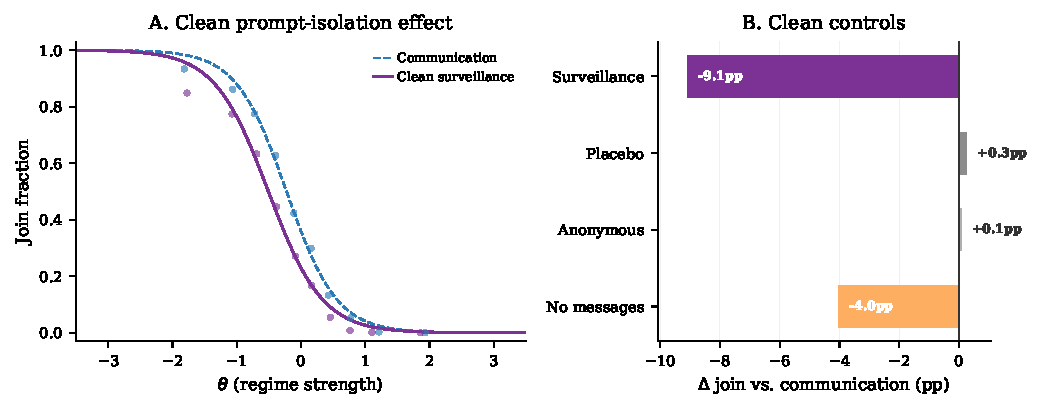
\includegraphics[width=0.94\textwidth]{../paper/figures/fig12_surveillance.pdf}

  \medskip
  \bigclaim{warn}{Participation falls when messages are monitored.}
\end{frame}

% 18 ------------------------------------------------------------------
\begin{frame}{Mechanism clue: beliefs do not move much}
  \Large
  The surprising part is not just lower action.\par
  \bigskip
  It is that stated beliefs about others' joining move much less than actions.

  \bigskip
  \centering
  \renewcommand{\arraystretch}{1.4}
  \begin{tabular}{@{}lcc@{}}
    \toprule
    & \textbf{Communication} & \textbf{Surveillance} \\
    \midrule
    Participation & higher & \bad{lower} \\
    Beliefs about others & similar & \ok{similar} \\
    \bottomrule
  \end{tabular}
\end{frame}

% 19 ------------------------------------------------------------------
\begin{frame}{What ``beliefs'' means here}
  \normalsize
  After choosing JOIN or STAY, each agent forecasts the crowd:\par

  \medskip
  \begin{block}{Second-order belief}
    \centering
    ``What fraction of the other citizens do you think will join the uprising?''
  \end{block}

  \smallskip
  \normalsize
  \begin{itemize}\setlength\itemsep{0.2em}
    \item A stated expectation about \hl{others' participation}.
    \item Not a direct readout of private type or true inner state.
    \item Measured after action, so I treat it as descriptive rather than a clean mediator.
  \end{itemize}

  \smallskip
  \begin{alertblock}{Key comparison}
    \small
    Do agents \textbf{act differently} while reporting similar beliefs?
  \end{alertblock}
\end{frame}

% 20 ------------------------------------------------------------------
\begin{frame}{Mechanism: monitored speech becomes less informative}
  \large
  Monitoring does not need to convince agents that the uprising is hopeless.\par
  \medskip
  It can work by making pro-uprising agents \bad{speak less clearly}.\par

  \medskip
  \begin{block}{Communication poisoning}
    \small
    The regime degrades the peer-information channel, so agents coordinate less even when their stated beliefs barely move.
  \end{block}
\end{frame}

% 21 ------------------------------------------------------------------
\begin{frame}{What monitoring does to speech}
  \begin{columns}[T]
    \begin{column}{0.48\textwidth}
      \begin{block}{Private signal}
        \large
        ``The regime's cohesion is visibly fraying.''\\[0.4em]
        ``Street talk has shifted from complaint to anticipation.''
      \end{block}
    \end{column}
    \begin{column}{0.48\textwidth}
      \begin{alertblock}{Message when monitored}
        \large
        ``Hard to know what will happen.''\\[0.4em]
        ``Best to stay cautious for now.''
      \end{alertblock}
    \end{column}
  \end{columns}

  \vspace{0.25cm}
  \centering
  {\LARGE\color{warn}\textbf{Monitored speech becomes less informative.}}\par

  \vspace{0.15cm}
  {\normalsize\color{muted}The extension turns a validation result into a stress test for coordination through language.}
\end{frame}

% 22 ------------------------------------------------------------------
\begin{frame}{What the evidence shows}
  \begin{enumerate}\setlength\itemsep{0.5em}
    \item \textbf{Baseline:} LLMs play the canonical global game in natural language.
    \item \textbf{Validation:} actions move with latent fundamentals, not generic sentiment.
    \item \textbf{Extension 1:} communication increases coordination.
    \item \textbf{Extension 2:} monitoring communication lowers participation.
    \item \textbf{Mechanism clue:} monitored speech changes more than stated beliefs.
  \end{enumerate}

  \medskip
  \centering\large\color{accent}\textbf{The general claim: LLMs can be used as controlled agents in language-rich global games.}
\end{frame}

% 22 ------------------------------------------------------------------
\begin{frame}[plain]
  \centering
  \vspace{1.2cm}
  {\Huge\color{purple}\textbf{Discussion.}}
\end{frame}

% =====================================================================
% Appendix: derivation kept out of the main talk
% =====================================================================
\appendix

\begin{frame}[plain]
  \centering
  \vspace{1.2cm}
  {\Huge\color{purple}\textbf{Appendix}}\\[0.8em]
  {\Large\color{muted}Solving the canonical global game}
\end{frame}

\begin{frame}{Appendix: complete information gives multiplicity}
  \small
  Normalize the attack payoff as
  \[
    u(1)=
    \begin{cases}
    1-c, & \text{if collapse occurs},\\
    -c, & \text{otherwise},
    \end{cases}
    \qquad u(0)=0,
    \qquad 0<c<1.
  \]

  \vspace{-0.1cm}
  If everyone observes $\theta$:
  \begin{itemize}\setlength\itemsep{0.25em}
    \item If everyone attacks, $A=1$ and collapse occurs for $\theta<1$.
    \item If nobody attacks, $A=0$ and collapse fails for $\theta>0$.
  \end{itemize}

  \smallskip
  \begin{block}{Multiplicity}
    For $0<\theta<1$, both $A=1$ and $A=0$ are self-confirming equilibria.
  \end{block}
\end{frame}

\begin{frame}{Appendix: cutoff strategy and aggregate attacks}
  \small
  Add private noisy signals:
  \[
    x_i=\theta+\sigma\varepsilon_i,
    \qquad \varepsilon_i\sim\mathcal N(0,1).
  \]

  Guess a monotone cutoff strategy:
  \[
    a_i(x_i)=
    \begin{cases}
    1, & x_i\le x^*,\\
    0, & x_i>x^*.
    \end{cases}
  \]

  Then, conditional on true $\theta$,
  \begin{align*}
    A(\theta)
    &=\Pr(x_i\le x^*\mid\theta)\\
    &=\Pr\left(\varepsilon_i\le \frac{x^*-\theta}{\sigma}\right)\\
    &=\Phi\left(\frac{x^*-\theta}{\sigma}\right).
  \end{align*}
\end{frame}

\begin{frame}{Appendix: boundary and marginal indifference}
  \small
  Collapse occurs when $A(\theta)\ge\theta$. The boundary fundamental $\theta^*$ solves
  \[
    \Phi\left(\frac{x^*-\theta^*}{\sigma}\right)=\theta^*.
  \]

  \smallskip
  At the cutoff, the marginal agent is indifferent:
  \[
    \Pr(\text{collapse}\mid x_i=x^*)=c.
  \]

  Since collapse occurs for $\theta\le\theta^*$,
  \[
    \Pr(\theta\le\theta^*\mid x_i=x^*)=c.
  \]

  With a diffuse prior and normal noise,
  \[
    \theta\mid x_i\sim\mathcal N(x_i,\sigma^2),
    \qquad
    \Phi\left(\frac{\theta^*-x^*}{\sigma}\right)=c.
  \]
\end{frame}

\begin{frame}{Appendix: clean solution}
  \footnotesize
  From marginal indifference,
  \[
    \Phi\left(\frac{\theta^*-x^*}{\sigma}\right)=c
    \quad\Rightarrow\quad
    x^*=\theta^*-\sigma\Phi^{-1}(c).
  \]

  \vspace{-0.15cm}
  Plug into the boundary equation:
  \begin{align*}
    \theta^*
    &=\Phi\left(\frac{x^*-\theta^*}{\sigma}\right)\\
    &=\Phi\left(-\Phi^{-1}(c)\right)=1-c.
  \end{align*}

  \vspace{-0.2cm}
  Therefore
  \[
    \theta^*=1-c,
    \qquad
    x^*=1-c-\sigma\Phi^{-1}(c).
  \]

  \vspace{-0.15cm}
  {\small\color{muted}\textbf{Takeaway:} private noise selects one threshold equilibrium: collapse below $\theta^*$, survival above it.}
\end{frame}

\begin{frame}{Appendix: empirical implication}
  \large
  The solved cutoff implies
  \[
    A(\theta)=\Phi\left(\frac{x^*-\theta}{\sigma}\right).
  \]

  \medskip
  Differentiating:
  \[
    \frac{dA(\theta)}{d\theta}
    =-\frac{1}{\sigma}\phi\left(\frac{x^*-\theta}{\sigma}\right)<0.
  \]

  \medskip
  \begin{block}{Validation target}
    \normalsize
    Higher assigned regime strength should produce lower LLM joining.
  \end{block}
\end{frame}

\end{document}
